\documentclass[11pt]{article}
\usepackage{enumitem}
\usepackage{latexsym}
\usepackage{amsfonts}
\usepackage{amsmath,amssymb,amsthm}
\usepackage{xcolor}
\usepackage{mathrsfs}
\usepackage{tikz}
\usepackage{hyperref}
\usetikzlibrary{arrows}
\usetikzlibrary{automata}

\setlength{\textheight}{8.5in}
\setlength{\textwidth}{6.0in}
\setlength{\headheight}{0in}
\addtolength{\topmargin}{-.5in}
\addtolength{\oddsidemargin}{-.5in}

%--------------
%% preamble.tex
%% this should be included with a command like
%% %--------------
%% preamble.tex
%% this should be included with a command like
%% %--------------
%% preamble.tex
%% this should be included with a command like
%% \input{preamble.tex}
%% \lecture{``lecture number''}{``date''}{``name of professor''}{``name
%%  of student''}
 
\hbadness=10000
\vbadness=10000
 
\newcommand{\handout}[5]{
   \renewcommand{\thepage}{#1-\arabic{page}}
   \noindent
   \begin{center}
   \framebox{
      \vbox{
    \hbox to 5.78in { {\bf CS 4510 Automata and Complexity
    	}
     	 \hfill #2 }
       \vspace{4mm}
       \hbox to 5.78in { {\Large \hfill #5  \hfill} }
       \vspace{2mm}
       \hbox to 5.78in { {\it #3 \hfill #4} }
      }
   }
   \end{center}
   \vspace*{4mm}
}
 
\newcommand{\lecture}[4]{\handout{#1}{#2}{Lecturer: #3}{Scribe(s): #4}{Lecture #1}}
\newcommand{\hw}[4]{\handout{#1}{#2}{#3}{#4}{Homework #1}}
\newcommand{\exam}[4]{\handout{#1}{#2}{#3}{#4}{Exam #1}}
 
 
 
 
\def\epsilon{\varepsilon}
\def\phi{\varphi}
\def\bool{\{0,1\}}
\def\poly{{\sf poly}}
\def\cross{\times}
 
\newcommand{\xor}{\oplus}
\newcommand{\Xor}{\bigoplus}
\newcommand{\ceil}[1]{\left\lceil {#1} \right\rceil}
\newcommand{\floor}[1]{\left\lfloor #1 \right\rfloor}
\newcommand{\ignore}[1]{}
%\newcommand{\integers}[1]{{\mathbb Z}_{#1}}
%\newcommand{\naturals}[1]{{\mathbb N}_{#1}}
\newcommand{\integers}{{\mathbb Z}}
\newcommand{\naturals}{{\mathbb N}}
\newcommand{\bydef}{\stackrel{\rm def}{=}}
\newcommand{\isequal}{\stackrel{\rm ?}{=}}
\newcommand{\compeq}{\stackrel{\rm c}{\equiv}} % computationally indistinguishable
 
%\newcommand{\qed}{\hspace*{\fill}\rule{7pt}{7pt}}
\newenvironment{proof_sketch}{\noindent{\bf Sketch of Proof} (Informal)\hspace*{1em}}{\qed\medskip}
%\newenvironment{proof}{\noindent{\bf Proof}\hspace*{1em}}{\qed\medskip}
\newenvironment{proofof}[1]{\noindent{\bf Proof} of #1:\hspace*{1em}}{\qed\medskip}
%\newenvironment{claim}{\noindent{\bf Claim}\hspace*{1em}\begin{em}}{\end{em}\medskip}
\newcounter{defcounter}
\setcounter{defcounter}{1}
\newenvironment{definition}{\medskip\noindent{\bf Definition \thedefcounter}}{\hspace*{\fill}$\diamondsuit$\stepcounter{defcounter}\medskip}
\newtheorem{theorem}{Theorem}
\newtheorem{corollary}[theorem]{Corollary}
\newtheorem{lemma}[theorem]{Lemma}
\newtheorem{claim}[theorem]{Claim}
\newtheorem{fact}[theorem]{Fact}
\newtheorem{conjecture}[theorem]{Conjecture}
\newenvironment{assumption}{\noindent{\bf Assumption}\hspace*{1em}\begin{em}}{\end{em}\medskip}
\newenvironment{remark}{\noindent{\bf Remark}\hspace*{1em}}{\bigskip}
 
\ignore{
\newcommand{\FOR}{{\bf for}}
\newcommand{\TO}{{\bf to}}
\newcommand{\DO}{{\bf do}}
\newcommand{\WHILE}{{\bf while}}
\newcommand{\AND}{{\bf and}}
\newcommand{\IF}{{\bf if}}
\newcommand{\THEN}{{\bf then}}
\newcommand{\ELSE}{{\bf else}}
 
%%% You probably will not need to use the commands listed below
 
\makeatletter
\def\fnum@figure{{\bf Figure \thefigure}}
\def\fnum@table{{\bf Table \thetable}}
\long\def\@mycaption#1[#2]#3{\addcontentsline{\csname
  ext@#1\endcsname}{#1}{\protect\numberline{\csname
  the#1\endcsname}{\ignorespaces #2}}\par
  \begingroup
    \@parboxrestore
    \small
    \@makecaption{\csname fnum@#1\endcsname}{\ignorespaces #3}\par
  \endgroup}
\def\mycaption{\refstepcounter\@captype \@dblarg{\@mycaption\@captype}}
\makeatother
 
\newcommand{\figcaption}[1]{\mycaption[]{#1}}
\newcommand{\tabcaption}[1]{\mycaption[]{#1}}
\newcommand{\head}[1]{\chapter[Lecture \##1]{}}
\newcommand{\mathify}[1]{\ifmmode{#1}\else\mbox{$#1$}\fi}
\def\half{\frac{1}{2}}
 
\newcommand{\fig}[4]{
        \begin{figure}
        \setlength{\epsfysize}{#2}
        \vspace{3mm}
        \centerline{\epsfbox{#4}}
        \caption{#3} \label{#1}
        \end{figure}
        }
}

%% \lecture{``lecture number''}{``date''}{``name of professor''}{``name
%%  of student''}
 
\hbadness=10000
\vbadness=10000
 
\newcommand{\handout}[5]{
   \renewcommand{\thepage}{#1-\arabic{page}}
   \noindent
   \begin{center}
   \framebox{
      \vbox{
    \hbox to 5.78in { {\bf CS 4510 Automata and Complexity
    	}
     	 \hfill #2 }
       \vspace{4mm}
       \hbox to 5.78in { {\Large \hfill #5  \hfill} }
       \vspace{2mm}
       \hbox to 5.78in { {\it #3 \hfill #4} }
      }
   }
   \end{center}
   \vspace*{4mm}
}
 
\newcommand{\lecture}[4]{\handout{#1}{#2}{Lecturer: #3}{Scribe(s): #4}{Lecture #1}}
\newcommand{\hw}[4]{\handout{#1}{#2}{#3}{#4}{Homework #1}}
\newcommand{\exam}[4]{\handout{#1}{#2}{#3}{#4}{Exam #1}}
 
 
 
 
\def\epsilon{\varepsilon}
\def\phi{\varphi}
\def\bool{\{0,1\}}
\def\poly{{\sf poly}}
\def\cross{\times}
 
\newcommand{\xor}{\oplus}
\newcommand{\Xor}{\bigoplus}
\newcommand{\ceil}[1]{\left\lceil {#1} \right\rceil}
\newcommand{\floor}[1]{\left\lfloor #1 \right\rfloor}
\newcommand{\ignore}[1]{}
%\newcommand{\integers}[1]{{\mathbb Z}_{#1}}
%\newcommand{\naturals}[1]{{\mathbb N}_{#1}}
\newcommand{\integers}{{\mathbb Z}}
\newcommand{\naturals}{{\mathbb N}}
\newcommand{\bydef}{\stackrel{\rm def}{=}}
\newcommand{\isequal}{\stackrel{\rm ?}{=}}
\newcommand{\compeq}{\stackrel{\rm c}{\equiv}} % computationally indistinguishable
 
%\newcommand{\qed}{\hspace*{\fill}\rule{7pt}{7pt}}
\newenvironment{proof_sketch}{\noindent{\bf Sketch of Proof} (Informal)\hspace*{1em}}{\qed\medskip}
%\newenvironment{proof}{\noindent{\bf Proof}\hspace*{1em}}{\qed\medskip}
\newenvironment{proofof}[1]{\noindent{\bf Proof} of #1:\hspace*{1em}}{\qed\medskip}
%\newenvironment{claim}{\noindent{\bf Claim}\hspace*{1em}\begin{em}}{\end{em}\medskip}
\newcounter{defcounter}
\setcounter{defcounter}{1}
\newenvironment{definition}{\medskip\noindent{\bf Definition \thedefcounter}}{\hspace*{\fill}$\diamondsuit$\stepcounter{defcounter}\medskip}
\newtheorem{theorem}{Theorem}
\newtheorem{corollary}[theorem]{Corollary}
\newtheorem{lemma}[theorem]{Lemma}
\newtheorem{claim}[theorem]{Claim}
\newtheorem{fact}[theorem]{Fact}
\newtheorem{conjecture}[theorem]{Conjecture}
\newenvironment{assumption}{\noindent{\bf Assumption}\hspace*{1em}\begin{em}}{\end{em}\medskip}
\newenvironment{remark}{\noindent{\bf Remark}\hspace*{1em}}{\bigskip}
 
\ignore{
\newcommand{\FOR}{{\bf for}}
\newcommand{\TO}{{\bf to}}
\newcommand{\DO}{{\bf do}}
\newcommand{\WHILE}{{\bf while}}
\newcommand{\AND}{{\bf and}}
\newcommand{\IF}{{\bf if}}
\newcommand{\THEN}{{\bf then}}
\newcommand{\ELSE}{{\bf else}}
 
%%% You probably will not need to use the commands listed below
 
\makeatletter
\def\fnum@figure{{\bf Figure \thefigure}}
\def\fnum@table{{\bf Table \thetable}}
\long\def\@mycaption#1[#2]#3{\addcontentsline{\csname
  ext@#1\endcsname}{#1}{\protect\numberline{\csname
  the#1\endcsname}{\ignorespaces #2}}\par
  \begingroup
    \@parboxrestore
    \small
    \@makecaption{\csname fnum@#1\endcsname}{\ignorespaces #3}\par
  \endgroup}
\def\mycaption{\refstepcounter\@captype \@dblarg{\@mycaption\@captype}}
\makeatother
 
\newcommand{\figcaption}[1]{\mycaption[]{#1}}
\newcommand{\tabcaption}[1]{\mycaption[]{#1}}
\newcommand{\head}[1]{\chapter[Lecture \##1]{}}
\newcommand{\mathify}[1]{\ifmmode{#1}\else\mbox{$#1$}\fi}
\def\half{\frac{1}{2}}
 
\newcommand{\fig}[4]{
        \begin{figure}
        \setlength{\epsfysize}{#2}
        \vspace{3mm}
        \centerline{\epsfbox{#4}}
        \caption{#3} \label{#1}
        \end{figure}
        }
}

%% \lecture{``lecture number''}{``date''}{``name of professor''}{``name
%%  of student''}
 
\hbadness=10000
\vbadness=10000
 
\newcommand{\handout}[5]{
   \renewcommand{\thepage}{#1-\arabic{page}}
   \noindent
   \begin{center}
   \framebox{
      \vbox{
    \hbox to 5.78in { {\bf CS 4510 Automata and Complexity
    	}
     	 \hfill #2 }
       \vspace{4mm}
       \hbox to 5.78in { {\Large \hfill #5  \hfill} }
       \vspace{2mm}
       \hbox to 5.78in { {\it #3 \hfill #4} }
      }
   }
   \end{center}
   \vspace*{4mm}
}
 
\newcommand{\lecture}[4]{\handout{#1}{#2}{Lecturer: #3}{Scribe(s): #4}{Lecture #1}}
\newcommand{\hw}[4]{\handout{#1}{#2}{#3}{#4}{Homework #1}}
\newcommand{\exam}[4]{\handout{#1}{#2}{#3}{#4}{Exam #1}}
 
 
 
 
\def\epsilon{\varepsilon}
\def\phi{\varphi}
\def\bool{\{0,1\}}
\def\poly{{\sf poly}}
\def\cross{\times}
 
\newcommand{\xor}{\oplus}
\newcommand{\Xor}{\bigoplus}
\newcommand{\ceil}[1]{\left\lceil {#1} \right\rceil}
\newcommand{\floor}[1]{\left\lfloor #1 \right\rfloor}
\newcommand{\ignore}[1]{}
%\newcommand{\integers}[1]{{\mathbb Z}_{#1}}
%\newcommand{\naturals}[1]{{\mathbb N}_{#1}}
\newcommand{\integers}{{\mathbb Z}}
\newcommand{\naturals}{{\mathbb N}}
\newcommand{\bydef}{\stackrel{\rm def}{=}}
\newcommand{\isequal}{\stackrel{\rm ?}{=}}
\newcommand{\compeq}{\stackrel{\rm c}{\equiv}} % computationally indistinguishable
 
%\newcommand{\qed}{\hspace*{\fill}\rule{7pt}{7pt}}
\newenvironment{proof_sketch}{\noindent{\bf Sketch of Proof} (Informal)\hspace*{1em}}{\qed\medskip}
%\newenvironment{proof}{\noindent{\bf Proof}\hspace*{1em}}{\qed\medskip}
\newenvironment{proofof}[1]{\noindent{\bf Proof} of #1:\hspace*{1em}}{\qed\medskip}
%\newenvironment{claim}{\noindent{\bf Claim}\hspace*{1em}\begin{em}}{\end{em}\medskip}
\newcounter{defcounter}
\setcounter{defcounter}{1}
\newenvironment{definition}{\medskip\noindent{\bf Definition \thedefcounter}}{\hspace*{\fill}$\diamondsuit$\stepcounter{defcounter}\medskip}
\newtheorem{theorem}{Theorem}
\newtheorem{corollary}[theorem]{Corollary}
\newtheorem{lemma}[theorem]{Lemma}
\newtheorem{claim}[theorem]{Claim}
\newtheorem{fact}[theorem]{Fact}
\newtheorem{conjecture}[theorem]{Conjecture}
\newenvironment{assumption}{\noindent{\bf Assumption}\hspace*{1em}\begin{em}}{\end{em}\medskip}
\newenvironment{remark}{\noindent{\bf Remark}\hspace*{1em}}{\bigskip}
 
\ignore{
\newcommand{\FOR}{{\bf for}}
\newcommand{\TO}{{\bf to}}
\newcommand{\DO}{{\bf do}}
\newcommand{\WHILE}{{\bf while}}
\newcommand{\AND}{{\bf and}}
\newcommand{\IF}{{\bf if}}
\newcommand{\THEN}{{\bf then}}
\newcommand{\ELSE}{{\bf else}}
 
%%% You probably will not need to use the commands listed below
 
\makeatletter
\def\fnum@figure{{\bf Figure \thefigure}}
\def\fnum@table{{\bf Table \thetable}}
\long\def\@mycaption#1[#2]#3{\addcontentsline{\csname
  ext@#1\endcsname}{#1}{\protect\numberline{\csname
  the#1\endcsname}{\ignorespaces #2}}\par
  \begingroup
    \@parboxrestore
    \small
    \@makecaption{\csname fnum@#1\endcsname}{\ignorespaces #3}\par
  \endgroup}
\def\mycaption{\refstepcounter\@captype \@dblarg{\@mycaption\@captype}}
\makeatother
 
\newcommand{\figcaption}[1]{\mycaption[]{#1}}
\newcommand{\tabcaption}[1]{\mycaption[]{#1}}
\newcommand{\head}[1]{\chapter[Lecture \##1]{}}
\newcommand{\mathify}[1]{\ifmmode{#1}\else\mbox{$#1$}\fi}
\def\half{\frac{1}{2}}
 
\newcommand{\fig}[4]{
        \begin{figure}
        \setlength{\epsfysize}{#2}
        \vspace{3mm}
        \centerline{\epsfbox{#4}}
        \caption{#3} \label{#1}
        \end{figure}
        }
}


\tikzset{
->, % makes the edges directed
>=stealth, % makes the arrow heads bold
node distance=4cm, % specifies the minimum distance between two nodes. Change if necessary.
every state/.style={thick, fill=gray!10}, % sets the properties for each ’state’ node
initial text=$ $, % sets the text that appears on the start arrow
}

\newcommand{\solution}[1]{\paragraph{Solution}  }
\newcommand{\bl}[1]{\textcolor{blue}{#1}}
\newcommand{\rd}[1]{\textcolor{red}{#1}}

\begin{document}
\hw{3: Turing Machines rev2}{2/17/2023}{DONT FORGET TO PUT YOUR NAME HERE}{Due:3/3/2023}

You should submit a typeset or \emph{neatly} written pdf on Gradescope.  The grading TA should not have to struggle to read what you've written; if your handwriting is hard to decipher, you will be asked to typeset your future assignments. Five bonus points if you use \LaTeX, and our template. You may collaborate with other students, but any written work should be your own. 

%CFGs, PDAs, pumping them
\begin{enumerate}
    \item Give the state diagram of a Turing machine which begins with $w\#$ on its tape for some $w \in \Sigma^*$ and halts with $w\#w$ on its tape. The input alphabet is $\Sigma = \{a,b\}$ and the tape alphabet may be $\Gamma = \{a,b,\dot{a}, \dot{b},\#,\textvisiblespace\}$.

    \solution{}

    $w \in \Sigma^* \qquad \Gamma = \{a,b,\dot{a}, \dot{b}, \#, \textvisiblespace\} \qquad \Sigma = \{a, b\}$

    \begin{figure}[ht]
        \centering
        \begin{tikzpicture}
            \node[state, initial] (q0) {$q_0$};
            \node[state, above of=q0] (q1) {$q_1$};
            \node[state, right of=q1] (q2) {$q_2$};
            \node[state, right of=q0] (q3) {$q_3$};
            \node[state, below of=q0, accepting] (q4) {$q_4$};
            
            \draw   

                (q0) edge[left] node{$a \rightarrow \dot{a}, R$} (q1)
                (q1) edge[loop above, above] node[text width=2cm, align=left]{$a \rightarrow a, R$ \\ $b \rightarrow b, R$ \\ $\# \rightarrow \#, R$} (q1)
                (q1) edge[above] node{$\textvisiblespace \rightarrow a, L$} (q2)
                (q2) edge[loop above, above] node[text width=2cm, align=left]{$a \rightarrow a, L$ \\ $b \rightarrow b, L$ \\ $\# \rightarrow \#, L$} (q2)
                (q2) edge[right] node[text width=2cm, align=right]{$\dot{a} \rightarrow a, R$ \\ $\dot{b} \rightarrow b, R $} (q0)

                (q0) edge[left] node{$\# \rightarrow \#, R$} (q4)

                (q0) edge[above] node{$b \rightarrow \dot{b}, R$} (q3)
                (q3) edge[loop below, below] node[text width=2cm, align=left]{$a \rightarrow a, R$ \\ $b \rightarrow b, R$ \\ $\# \rightarrow \#, R$} (q3)
                (q3) edge[bend right, right] node{$\textvisiblespace \rightarrow b, L$} (q2)

                ;
        \end{tikzpicture}
    \end{figure}

    \newpage

    \item Give the sequence of configurations of your state diagram beginning from $q_0aba\#$

    \solution{}
    
    $$q_0aba\#\textvisiblespace\textvisiblespace\textvisiblespace\textvisiblespace\textvisiblespace$$
    $$\dot{a}q_1ba\#\textvisiblespace\textvisiblespace\textvisiblespace\textvisiblespace\textvisiblespace$$
    $$\dot{a}bq_1a\#\textvisiblespace\textvisiblespace\textvisiblespace\textvisiblespace\textvisiblespace$$
    $$\dot{a}baq_1\#\textvisiblespace\textvisiblespace\textvisiblespace\textvisiblespace\textvisiblespace$$
    $$\dot{a}ba\#q_1\textvisiblespace\textvisiblespace\textvisiblespace\textvisiblespace\textvisiblespace$$
    $$\dot{a}baq_2\#a\textvisiblespace\textvisiblespace\textvisiblespace\textvisiblespace$$
    $$\dot{a}bq_2a\#a\textvisiblespace\textvisiblespace\textvisiblespace\textvisiblespace$$
    $$\dot{a}q_2ba\#a\textvisiblespace\textvisiblespace\textvisiblespace\textvisiblespace$$
    $$q_2\dot{a}ba\#a\textvisiblespace\textvisiblespace\textvisiblespace\textvisiblespace$$
    $$aq_0ba\#a\textvisiblespace\textvisiblespace\textvisiblespace\textvisiblespace$$
    $$a\dot{b}q_3a\#a\textvisiblespace\textvisiblespace\textvisiblespace\textvisiblespace$$
    $$a\dot{b}aq_3\#a\textvisiblespace\textvisiblespace\textvisiblespace\textvisiblespace$$
    $$a\dot{b}a\#q_3a\textvisiblespace\textvisiblespace\textvisiblespace\textvisiblespace$$
    $$a\dot{b}a\#aq_3\textvisiblespace\textvisiblespace\textvisiblespace\textvisiblespace$$
    $$a\dot{b}a\#q_2ab\textvisiblespace\textvisiblespace\textvisiblespace$$
    $$a\dot{b}aq_2\#ab\textvisiblespace\textvisiblespace\textvisiblespace$$
    $$a\dot{b}q_2a\#ab\textvisiblespace\textvisiblespace\textvisiblespace$$
    $$aq_2\dot{b}a\#ab\textvisiblespace\textvisiblespace\textvisiblespace$$
    $$abq_0a\#ab\textvisiblespace\textvisiblespace\textvisiblespace$$
    $$ab\dot{a}q_1\#ab\textvisiblespace\textvisiblespace\textvisiblespace$$
    $$ab\dot{a}\#q_1ab\textvisiblespace\textvisiblespace\textvisiblespace$$
    $$ab\dot{a}\#aq_1b\textvisiblespace\textvisiblespace\textvisiblespace$$
    $$ab\dot{a}\#abq_1\textvisiblespace\textvisiblespace\textvisiblespace$$
    $$ab\dot{a}\#aq_2ba\textvisiblespace\textvisiblespace$$
    $$ab\dot{a}\#q_2aba\textvisiblespace\textvisiblespace$$
    $$ab\dot{a}q_2\#aba\textvisiblespace\textvisiblespace$$
    $$abq_2\dot{a}\#aba\textvisiblespace\textvisiblespace$$
    $$abaq_0\#aba\textvisiblespace\textvisiblespace$$
    $$aba\#q_4aba\textvisiblespace\textvisiblespace$$
    
    \item Give a high level, detailed, description of a Turing machine which computes the projection function $U(n,i,x_1,x_2,...,x_n) = x_i$.

    You get to choose, within reason, the initial encoding of the input on the tape. The Turing machine must halt with just $x_i$ on its tape leftshifted as much as possible. If this was psuedocode, the Turing machine would compute the following algorithm:
    \begin{verbatim}
        def U(n, i, A):
            return A[i]
    \end{verbatim}

    \solution{} Let $\beta$ be the set of all characters in any of the $x_k \forall k$. That is, $$x_k \in \beta^* \quad \forall \quad k=1,2,\dots,n$$
    Further, let $\alpha = \mathbb{N} \cup [0, N] = 0, 1, 2, \dots, N$ where $N$ is the maximum length string we are allowing to handle. For simplicity, we assume $\beta \cap \alpha = \emptyset$ since if $\beta$ includes any numbers, we can just make up symbols to use to represent each number (e.g. $n_k$ is $k$). 

    Then let $\Sigma = \{\#\} \cup \alpha \cup \beta$ and $\Gamma = \Sigma \cup \{\textvisiblespace\}$.

    Let the initial configuration on the tape be:

    $$q_0ix_1\#x_2\#x_3\#\dots\#x_n$$

    where $i \in \Sigma$, but $x_k \in \Sigma^* \forall k$.

    Do $U$ on $ix_1\#x_2\#x_3\#\dots\#x_n\textvisiblespace\textvisiblespace\textvisiblespace\dots$:

    \begin{enumerate}
        \item Decrement $i$ and move right. This is done using transitions of the form $k \rightarrow k-1, R \quad \forall \quad k \in \alpha$
        \item Set the tape location to $\textvisiblespace$ (clearing it) and move right while you see symbols in $\beta$
        \item Once $\#$ is reached, clear it (set to $\textvisiblespace$) and move left
        \item loop left (without changing anything) back to the $i$
        \item Go back to step a if $i \neq 0$, if $i = 0$ continue to step f
        \item loop right past all the $\textvisiblespace$
        \item loop right past all the $\beta$ characters
        \item When you see $\textvisiblespace$ or $\#$, move left to the last $\beta$ character while writing $\#$ (even when $\textvisiblespace$ was seen).
        \item Shift everything to the left by one unit by copying each character to the position on the left. For the first write, use a $\#$ to clear the last character. For each character, store it into the states, and then move left and write it, again storing the overriden character in the state. Repeat this until you see either $0$ or $\textvisiblespace$.
        \item If you saw $\textvisiblespace$, we have successfully shifted the word by one unit, and we must repeat this by going back to step g, otherwise continue to step k
        \item At this point the tape should look like this
            $$x_i\#\dots\#x_{i+1}\#\dots\#x_n$$
        So we just loop to the first $\#$ to clean up the ending
        \item Clear everything to the right of (and including) the first $\#$ by setting it to $\textvisiblespace$. Once a $\textvisiblespace$ is found on the tape, complete the computation by entering a final state.
    \end{enumerate}

    That should outline the Turing Machine. NOTE: the rest of the stuff below is extra.

    Here is the turing machine state diagram:
    \begin{center}
        \centering
        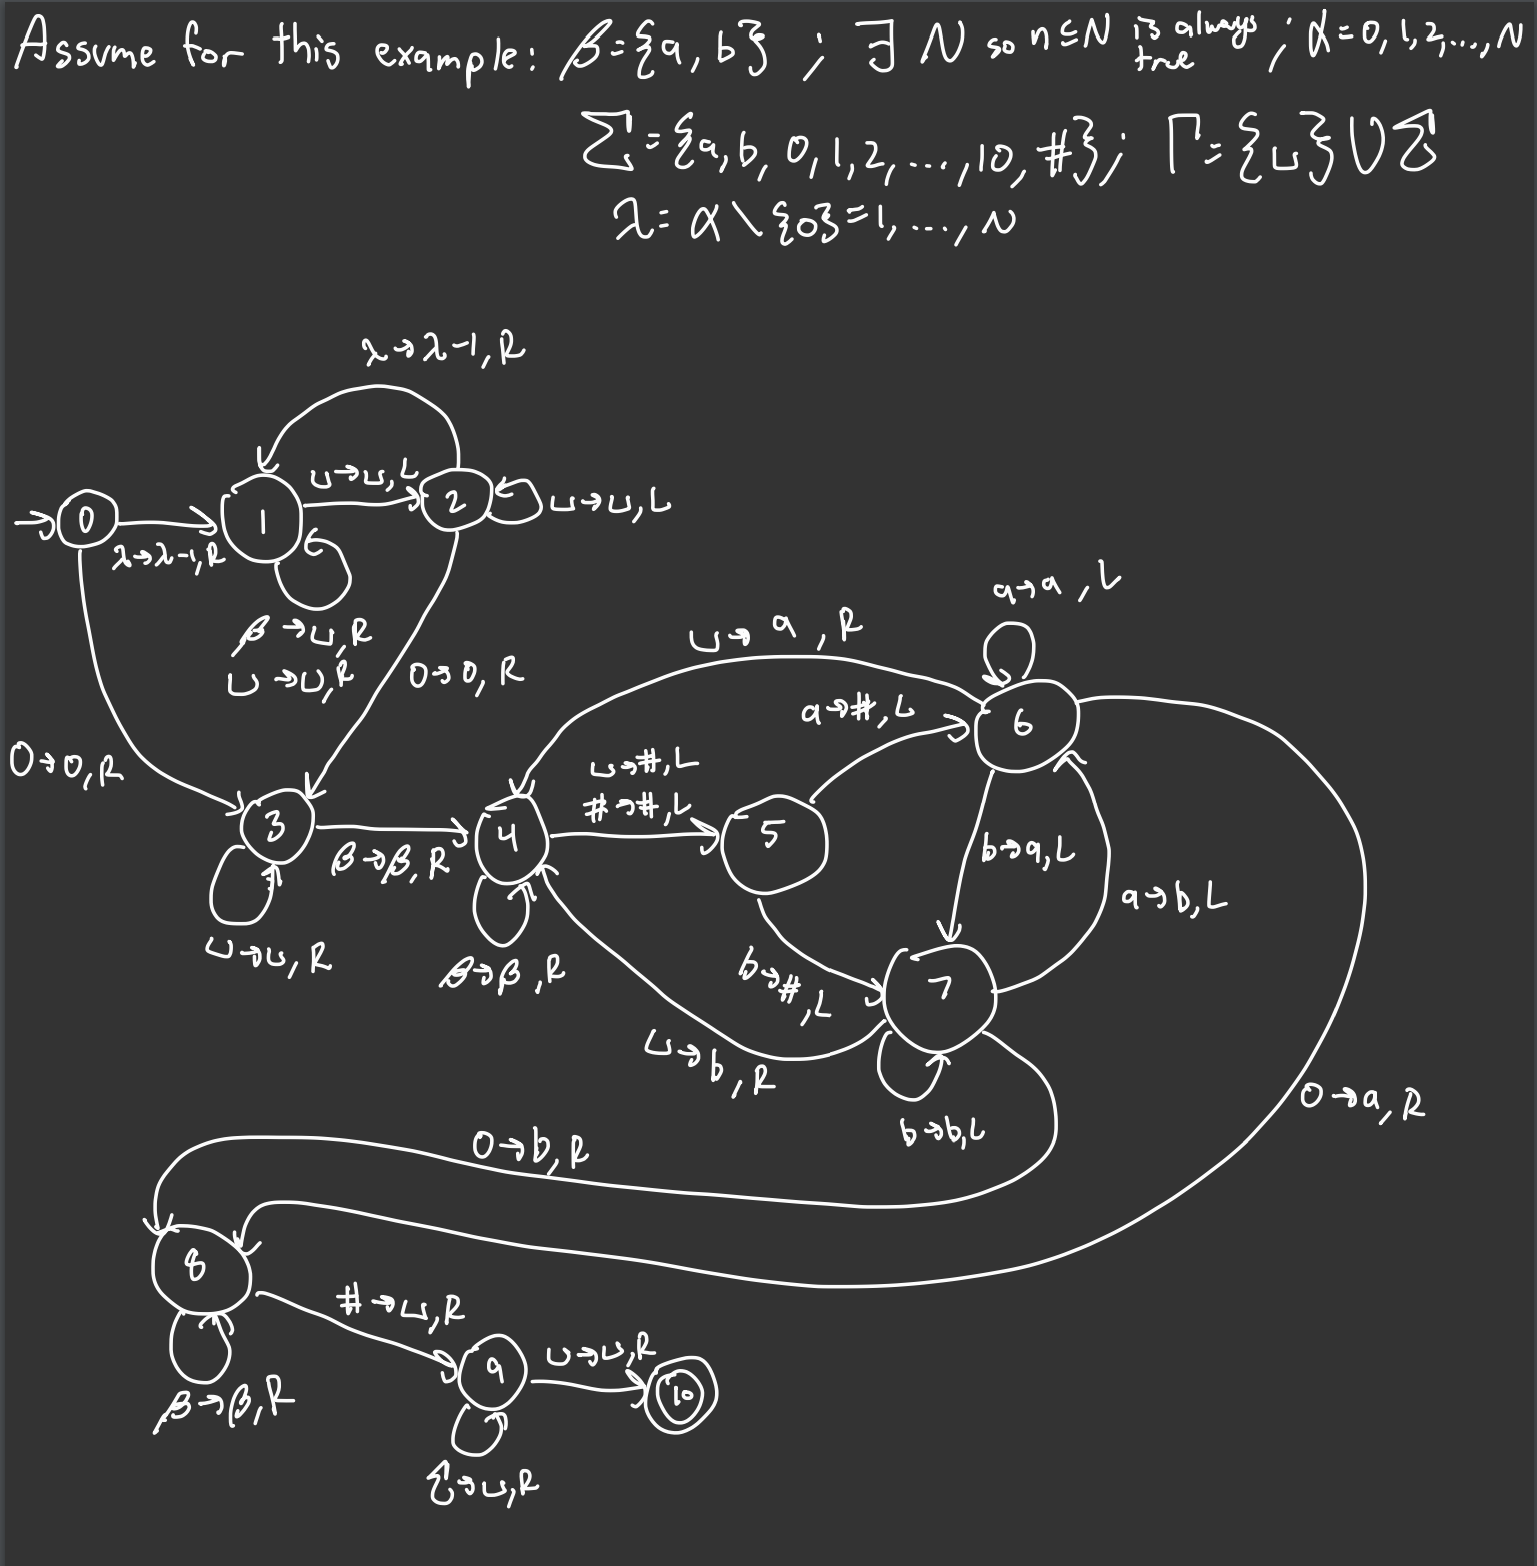
\includegraphics[width=0.9\textwidth]{HW3/res/index_tm.png}
        \label{fig:my_label}
    \end{center}
    The turing machine state diagram for the index operation outlined above. Note that the states are labelled 0,1,2,\dots,10 instead of $q_0,\dots,q_10$. This turing machine was loaded into a simulator I made and gave these results: $$2aabaaa\#abbaa\#bba\#aab\#aaa \rightarrow bba$$

    which is as expected. See \href{https://github.com/rishavb123/TuringMachineSimulator/blob/f09c4615af96bd1018fafee31a0e7781b3dcd43a/tm/examples.py#L61}{here} for the code.

    \item Oops. We took a Turing machine and dropped it the gears are broken or slipping or something. Instead of moving one unit left, or one unit right. It can now move only $l$ units left or $r$ units right. Prove that if $gcd(l,r) = 1$ then our broken $(l,r)$-machine is still Turing complete. Discuss how it could kind of still be Turing-complete if $l,r$ were not relatively prime. As a warmup, consider an $(2,3)$-machine.

    \solution{} Without loss of generality, let $l > r$. If $r \geq l$, just do the same proof with $l$ and $r$ switched. First, we can run the Euclidean Algorithm to calculate the GCD of $l$ and $r$, which should give us 1 in this case as follows:

    $$\exists \quad a, b \in \mathbb{N} \qquad l = ar + b \qquad l > r, r > b $$ $$ b = l - ar$$
    $$\exists \quad c, d \in \mathbb{N} \qquad r = cb + d \qquad r > b, b > d $$ $$ d = r - cb$$
    $$\exists \quad e, f \in \mathbb{N} \qquad b = ed + f \qquad b > d, d > f $$ $$ f = b - ed = (e - ea - a)r + (1 - c)l$$
    $$\vdots$$
    This eventually gets us to the GCD of the two numbers which we can then write as a linear combination of $r$ and $l$ using the same method that we found a linear combination of $b$, $d$, and $f$. Thus,
    $$\exists \quad m, n \in \mathbb{N} \qquad \gcd(l, r) = mr + nl \qquad mn < 0$$
    
    
    If $m > 0$ and $n < 0$, let $k = -n$, so $k > 0$
    $$l = mr - kl$$
    To produce $-1$, we can do this,
    $$-1 = (l - 1) - l$$
    $$l - 1 = (l-1)(1) = (l-1)mr - (l-1)kl$$
    $$-1 = (l-1)mr - (l-1)kl - l = [(l - 1)m]r - [(l-1)k - 1]l$$
    We can clearly already produce a single unit right with $m$ steps of length $r$ to the right and then $k$ steps of length $l$ to the left ($1 = mr-kl$). Now, we just showed that we can do the same for a single unit left with $(l - 1)m$ steps right of length $r$ and $(l-1)k - 1$ steps left of length $l$. So, we can effectively move right and left one unit on the tape in this case.

    If $m < 0$ and $n > 0$, let $k = -m$, so $k > 0$
    $$1=-kr+nl$$
    $$-1=kr-nl$$
    To produce $1$, we can do this,
    $$1 = -1(r-1)+r$$
    $$1 = (r-1)(kr-nl)+r$$
    $$1 = [(r-1)k + 1]r - [(r-1)n]l$$
    So similarly, we can produce $-1$ and $1$ for this case and move left or right on the tape using different combinations of the $l$ and $r$ steps.

    Thus, we can basically use the tape as normal, except every time we need to move left or right we call the subroutine to do so defined by the number of steps given from the equations above. Further, even if the GCD is not one, we can make the same argument from above to show that we can move $g = gcd(l, r)$ to the left or right. Then, we can perform whatever computations that a regular Turing Machine would do, but only using the locations on the tape that land on multiples of $g$. That is if we would have written to index $i$, we now write to index $ki$. If we move $1$ unit right or left, now we move $g$ units right or left.
    
    

    \item Prove that $\mathscr{L}(NFA)$ is countable.

    There are two ways we can prove this:

    1) The languages that can be represented by NFAs are the same languages that can be represented by regular expressions. Regular expressions have finite string representations, so by the Type writer principle, this set is countable.

    2) The languages that can be represented by NFAs are the same languages that can be represented by DFAs. In a DFA, there are finite number of states $|Q| < |\mathbb{N}|$ which can be arbitrarily large, but not infinite. Each state has $|\Sigma| < |\mathbb{N}|$ outbound edges, which is also finite. So the number of DFAs with length $|Q| = N$ is $N\cdot|\Sigma|$. This makes the total number of DFAs:
    $$\sum_{N \in \mathbb{N}}N|\Sigma| \leq |\mathbb{N}|(|\mathbb{N}||\Sigma|) \leq |\mathbb{N}||\mathbb{N}||\mathbb{N}| = |\mathbb{N}|^3 = |\mathbb{N}|$$
    The last step was proven in lecture.
    Thus $\mathscr{L}(NFA) = \mathscr{L}(DFA) = |\mathbb{N}|$ and $\mathscr{L}(NFA)$ is countable.

    
    \item Recall the definition of a DIA from the first homework. Prove that the set of all DIAs is uncountable. Lets clarify the definition of a DIA. $Q$ is countably infinite. $F\subseteq Q$ is finite or countably infinite. $\Sigma$ is finite. $\delta$ is defined appropriately for countably infinite $Q$ and finite $\Sigma$. 

    On the first homework, we showed that $\mathscr{L}(DIA)$ is the set of all languages, since a DIA can represent any language. Note that a language by definition is the set of all subsets of $\Sigma^*$. Thus, the set of all languages is just the power set of $\Sigma^*$, $\mathcal{P}(\Sigma^*)$. In lecture, we discussed that $\Sigma^*$ is countably infinite since $|\Sigma|$ is finite. So, $|\Sigma^*| = |\mathbb{N}|$.

    Now, by Cantor's Theorem,
    $$|\Sigma^*| < |\mathcal{P}(\Sigma^*)|$$
    So, 
    $$|\mathcal{P}(\Sigma^*)| = |\mathscr{L}(DIA)| > |\Sigma^*| = |\mathbb{N}|$$
    So,
    $$|\mathscr{L}(DIA)| > |\mathbb{N}|$$
    which proves that $\mathscr{L}(DIA)$ is uncountable.
\end{enumerate} 
\end{document}
